\chapter{Design Alternatives}

To identify a solution that balances performance, cost efficiency, and long-term sustainability, several design alternatives were assessed for technical feasibility, constructability, operational reliability, and regulatory compliance. The following sections present a focused comparison of these alternatives and culminate in the selection of the most appropriate option for the subdivision.

\section{Alternative 1 – Duplex Submersible Pump Station with PVC Force Main}\label{sec:alt1}

\subsection{Description}
This configuration consists of a below-grade circular wet well equipped with two submersible wastewater pumps arranged in a duty-standby setup. Each pump operates automatically based on preset wet-well levels detected by float switches or a pressure transducer. The pumped flow is conveyed through a pressurized force main that follows the subdivision roadway corridor to connect with the existing downstream gravity sewer system. The wet-well structure, valve vault, and electrical control panel are typically housed within a compact easement at the low point of the subdivision. This configuration represents the standard lift-station arrangement used in small residential developments where gravity flow is not possible throughout the service area.

\begin{figure}[H]
    \centering
    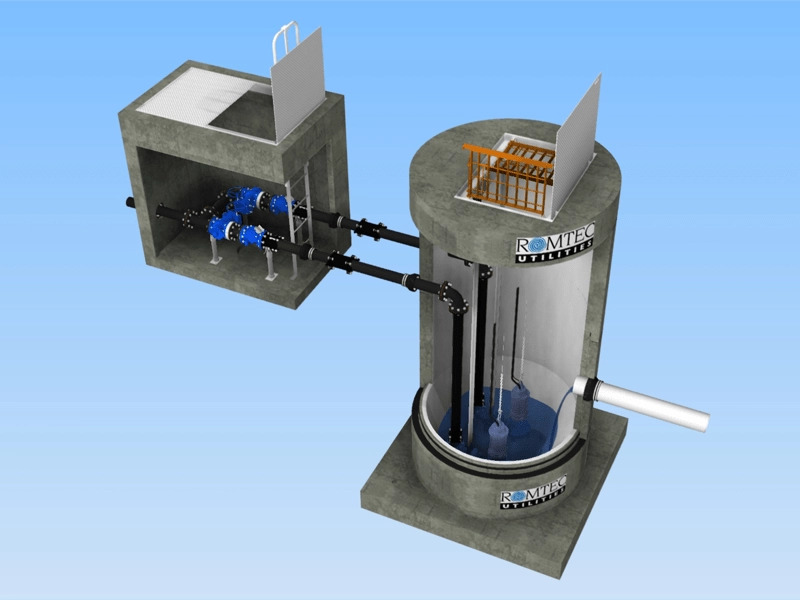
\includegraphics[width=0.75\textwidth]{alternative_1b.JPG}
    \caption{Three-dimensional rendering of a duplex submersible lift station showing wet well, pumps, and valve vault arrangement \cite{Romtec_StandardDuplex_LiftStation}.}
    \label{fig:alternative1_a}
\end{figure}

\subsection{Typical Application in Practice}
Duplex submersible pump stations are widely used by municipalities and developers for residential subdivisions across Mississippi. They provide centralized wastewater conveyance with redundancy, meeting state and local regulatory expectations for public ownership and maintenance under MDEQ’s \textit{Guidance for the Design of Publicly Owned Wastewater Facilities}~\cite{MDEQ_DesignGuidance_2025}.

\begin{figure}[H]
    \centering
    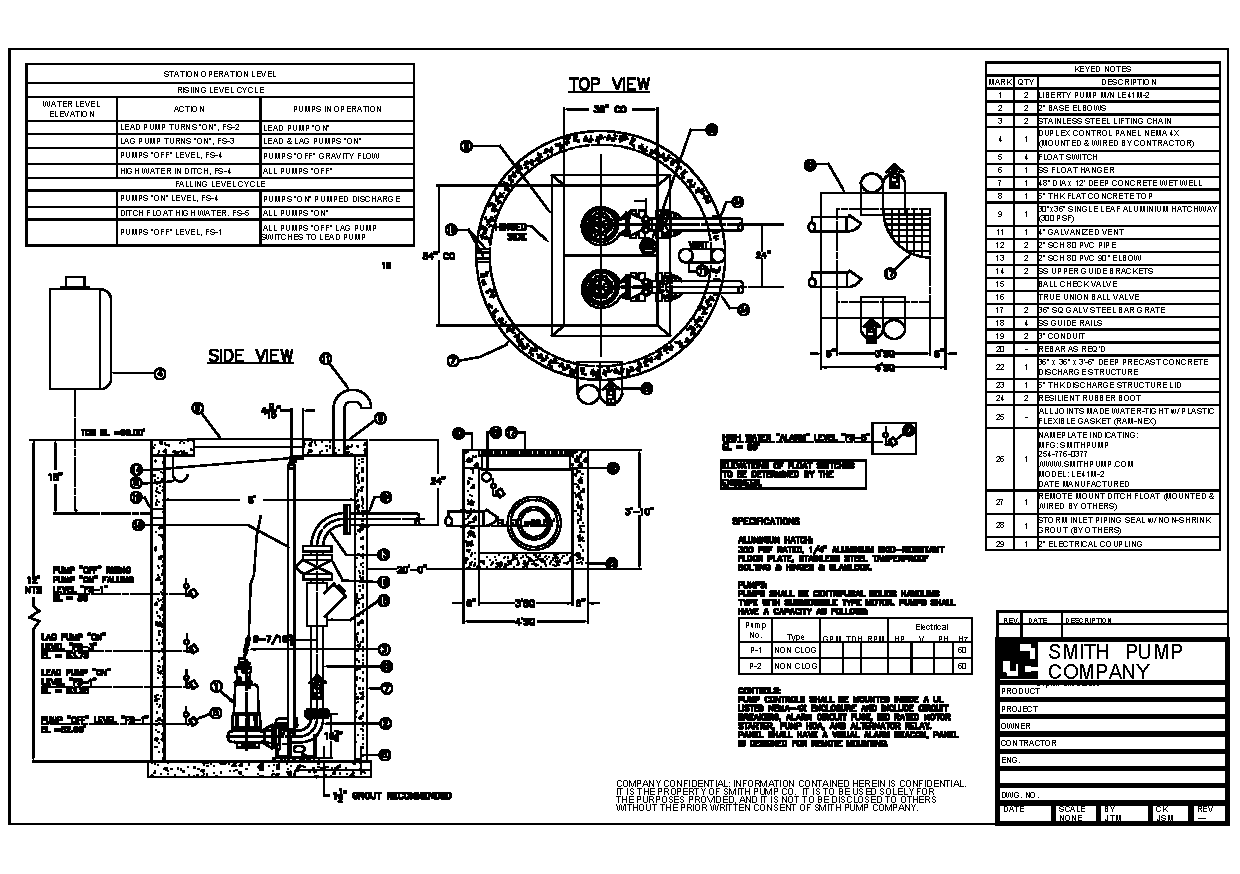
\includegraphics[width=1\textwidth]{alternative1b.pdf}
    \caption{Typical engineering drawing of a duplex submersible pump station with plan and section views, showing float controls, valves, and discharge piping layout \cite{SmithPump_DuplexSubmersible_LiftStation}.}
    \label{fig:alternative_1b}
\end{figure}

\subsection{Advantages}

The duplex submersible lift station offers high reliability through its redundant configuration. One pump remains on standby while the other operates under normal flow conditions, ensuring uninterrupted service during maintenance or in the event of a mechanical failure. This redundancy meets MDEQ’s requirements for small community wastewater systems and provides operational confidence for residential developments~\cite{MDEQ_DesignGuidance_2025}. The system also occupies a compact footprint, with most components installed below grade, minimizing land requirements and visual impact within the subdivision.

From an operational standpoint, municipal maintenance crews are highly familiar with this type of lift station, which simplifies inspection, troubleshooting, and part replacement. The station’s mechanical and electrical components are standard across many municipal systems, promoting ease of integration with existing maintenance programs. In terms of cost, this configuration provides a moderate initial investment compared to deep-gravity or distributed grinder systems while offering a lower life-cycle cost due to consolidated maintenance and shared control systems. The design is also expandable, as both the wet well and control panel can accommodate minor future flow increases without major reconstruction, making it a flexible and scalable solution for growing residential areas.

\subsection{Disadvantages}

The main disadvantage of the duplex submersible lift station lies in its mechanical and electrical dependence. Continuous power supply is required to sustain operation, meaning that outages can interrupt service unless backup power or emergency storage capacity is provided~\cite{NFPA_70_2023}. The system also faces potential odor and corrosion issues due to the accumulation of gases such as hydrogen sulfide within the wet well. Without adequate ventilation, coating, and chemical control, these gases can deteriorate structural and mechanical components over time~\cite{TenStates_RecommendedStandards_2014}.

Routine maintenance is another consideration, as the pumps, valves, and level sensors require regular inspection, lubrication, and periodic replacement. Although the duplex arrangement reduces the likelihood of total system downtime, the station still functions as a single point of failure for the subdivision. A complete station malfunction, while unlikely, would temporarily interrupt wastewater conveyance until repairs are completed. These limitations highlight the need for preventive maintenance, corrosion protection, and standby power provisions in the final design.

\subsection{Technical, Economic, Environmental, and Social Considerations}

From a technical perspective, the duplex submersible configuration provides consistent hydraulic performance by matching system flow and head requirements through controlled pumping operation. The system is capable of maintaining stable performance under both average and peak flow conditions while satisfying standard requirements for redundancy and wet-well capacity~\cite{MDEQ_DesignGuidance_2025,TenStates_RecommendedStandards_2014}. Economically, the lift station represents a balanced investment with moderate initial costs and predictable long-term maintenance expenses due to the use of centralized equipment and standardized components.

Environmentally, the system’s pressurized conveyance and sealed construction minimize the potential for exfiltration or infiltration, protecting both groundwater and surface water quality~\cite{EPA_LiftStation_DesignManual_2004}. The inclusion of proper ventilation and odor control also limits atmospheric emissions. Socially, the below-grade design reduces noise, odor, and visual impact, maintaining the residential character of the subdivision. Routine maintenance activities can be performed without major disruption to nearby residents, making this alternative both technically viable and socially acceptable for the Colebrooke Subdivision.


\section{Alternative 2 – Grinder Pump / Low-Pressure Sewer System}\label{sec:alt2}

\subsection{Description}
In this alternative, each residence, or in some cases a small cluster of homes, is equipped with an individual grinder-pump basin. The grinder pump collects wastewater from the house, grinds solids into a fine slurry, and discharges it through a small-diameter pressure service line into a shared low-pressure network that conveys flow to the downstream municipal sewer. The network typically consists of 1½- to 4-inch PVC or HDPE force mains operating under variable pressure. Check valves, isolation valves, and service connections are distributed throughout the subdivision rather than concentrated at a single central pump station~\cite{CFPUA_ResidentialGrinderPump_Diagram, LakesideMUD_LowPressureGrinderPump_SewerLayout}.

\begin{figure}[H]
    \centering
    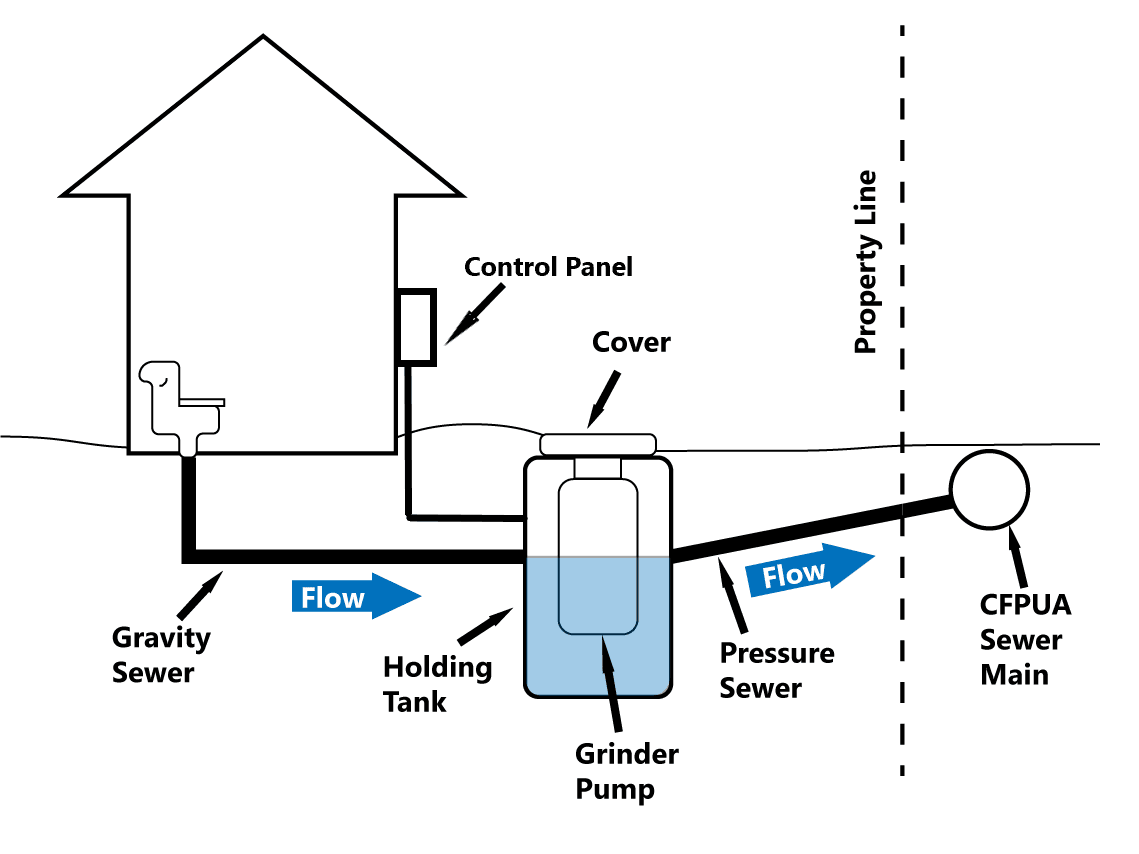
\includegraphics[width=0.8\textwidth]{alternative2a.png}
    \caption{Typical schematic of a household grinder-pump installation showing the holding tank, control panel, and connection to the low-pressure main~\cite{CFPUA_ResidentialGrinderPump_Diagram}.}
    \label{fig:alternative2a}
\end{figure}

\subsection{Typical Application in Practice}
Low-pressure grinder systems are commonly implemented in rural, hilly, or rocky areas where conventional gravity sewers would require deep excavation or multiple lift stations. They are also effective in regions with high groundwater tables or shallow rock, minimizing infiltration and exfiltration risks~\cite{EPA_LiftStation_DesignManual_2004}.

\begin{figure}[H]
    \centering
    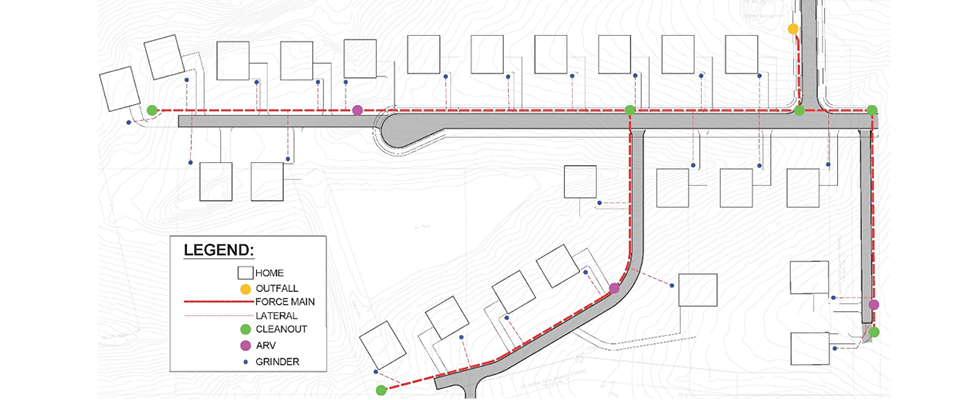
\includegraphics[width=1.05\textwidth]{alternative2b.png}
    \caption{Example layout of a low-pressure grinder-pump network in a residential subdivision, illustrating individual service laterals, shared force mains, and outfall connection~\cite{LakesideMUD_LowPressureGrinderPump_SewerLayout}.}
    \label{fig:alternative2b}
\end{figure}

\subsection{Advantages}

The grinder pump and low-pressure sewer system offers several advantages for small residential developments such as the Colebrooke Subdivision. The most notable benefit is the elimination of a central pump station, which removes the need for a large wet well, electrical control building, and associated mechanical infrastructure. This simplifies the overall system layout and reduces upfront construction costs. The system also allows for shallow installation, following natural surface grades with minimal trench depth. This characteristic reduces excavation costs, limits disturbance to existing soils, and minimizes potential conflicts with groundwater or unsuitable subgrade materials.

Another key advantage is the system’s flexibility in alignment. The small-diameter pressure mains can be routed around existing utilities, landscaping, or terrain constraints without major redesign, making it ideal for irregular or developed sites. The scalability of the system also supports incremental expansion; additional residences can be connected with minimal disruption or system modification. Furthermore, localized failures are limited in impact, as a malfunction typically affects only the individual home or a small group of houses served by that particular grinder pump, rather than the entire subdivision. This distributed configuration enhances overall system resilience and reduces the risk of widespread service interruption.

\subsection{Disadvantages}

Despite its flexibility, the grinder pump and low-pressure sewer system presents several drawbacks when applied to a small residential development. The most significant limitation is the requirement for multiple mechanical units, as each home must be equipped with its own grinder pump, float controls, and electrical connection. This greatly increases the total number of components to install, monitor, and maintain. Over time, this distributed setup can lead to higher cumulative maintenance costs compared to a centralized lift station.

Another major concern involves ownership and maintenance responsibility. It is often unclear whether individual homeowners, homeowners’ associations, or the municipality are responsible for servicing the pumps. This ambiguity can create management and liability challenges, especially in privately owned subdivisions. The system is also highly dependent on residential power supply, since each grinder unit relies on the homeowner’s electrical connection. During power outages, the basin provides only limited short-term storage capacity~\cite{NFPA_70_2023}.

Additional drawbacks include potential noise and odor issues if basins are not properly sealed or ventilated, particularly given their proximity to occupied dwellings. Furthermore, because each unit operates independently, the lifespan of pumps and controls may vary, resulting in non-uniform replacement cycles and complicating maintenance scheduling. Collectively, these disadvantages make long-term operation and management more complex than in a single centralized pumping system.

\subsection{Technical, Economic, Environmental, and Social Considerations}

From a technical standpoint, the grinder pump and low-pressure sewer system maintains adequate flow velocity within small-diameter pressure lines, effectively conveying wastewater with minimal sedimentation risk. However, the system’s performance depends heavily on the consistent operation of each individual pump. If one or more pumps fail, localized service interruptions or reduced conveyance efficiency may occur~\cite{EPA_LiftStation_DesignManual_2004}.

In economic terms, installation costs per home are often comparable to or slightly lower than those of a conventional gravity sewer, primarily due to the reduced excavation depth and smaller pipe diameters. However, the distributed nature of the system results in higher long-term operation and maintenance costs, as each home contains a separate pump, control system, and power source that must be individually serviced.

From an environmental perspective, the shallow and flexible installation minimizes excavation and overall land disturbance. Despite this advantage, the presence of multiple small pump basins increases the number of potential overflow points, especially during power outages or equipment failures.

In social terms, this configuration may be less preferred in planned residential developments where centralized municipal management of wastewater infrastructure is desired. The need for individual maintenance and the presence of mechanical equipment on private property can introduce management complexity and variability in system performance across users.

\section{Alternative 3 – Deep Gravity Sewer System}\label{sec:alt3}

\subsection{Description}
This alternative eliminates the need for a pump station by constructing a deep gravity sewer network that allows wastewater to flow naturally toward the downstream collection system. Achieving this configuration would require lowering the outlet elevation at the subdivision discharge point and installing deeper manholes and pipes along the main alignment. The design involves larger excavation depths, strict trench safety measures, and the use of suitable bedding materials to maintain pipe stability and prevent settlement. In areas with soft or saturated clay soils, shoring and dewatering would be necessary to ensure construction safety and long-term performance, as illustrated in Figure~\ref{fig:alternative3a}. 

\begin{figure}[H]
    \centering
    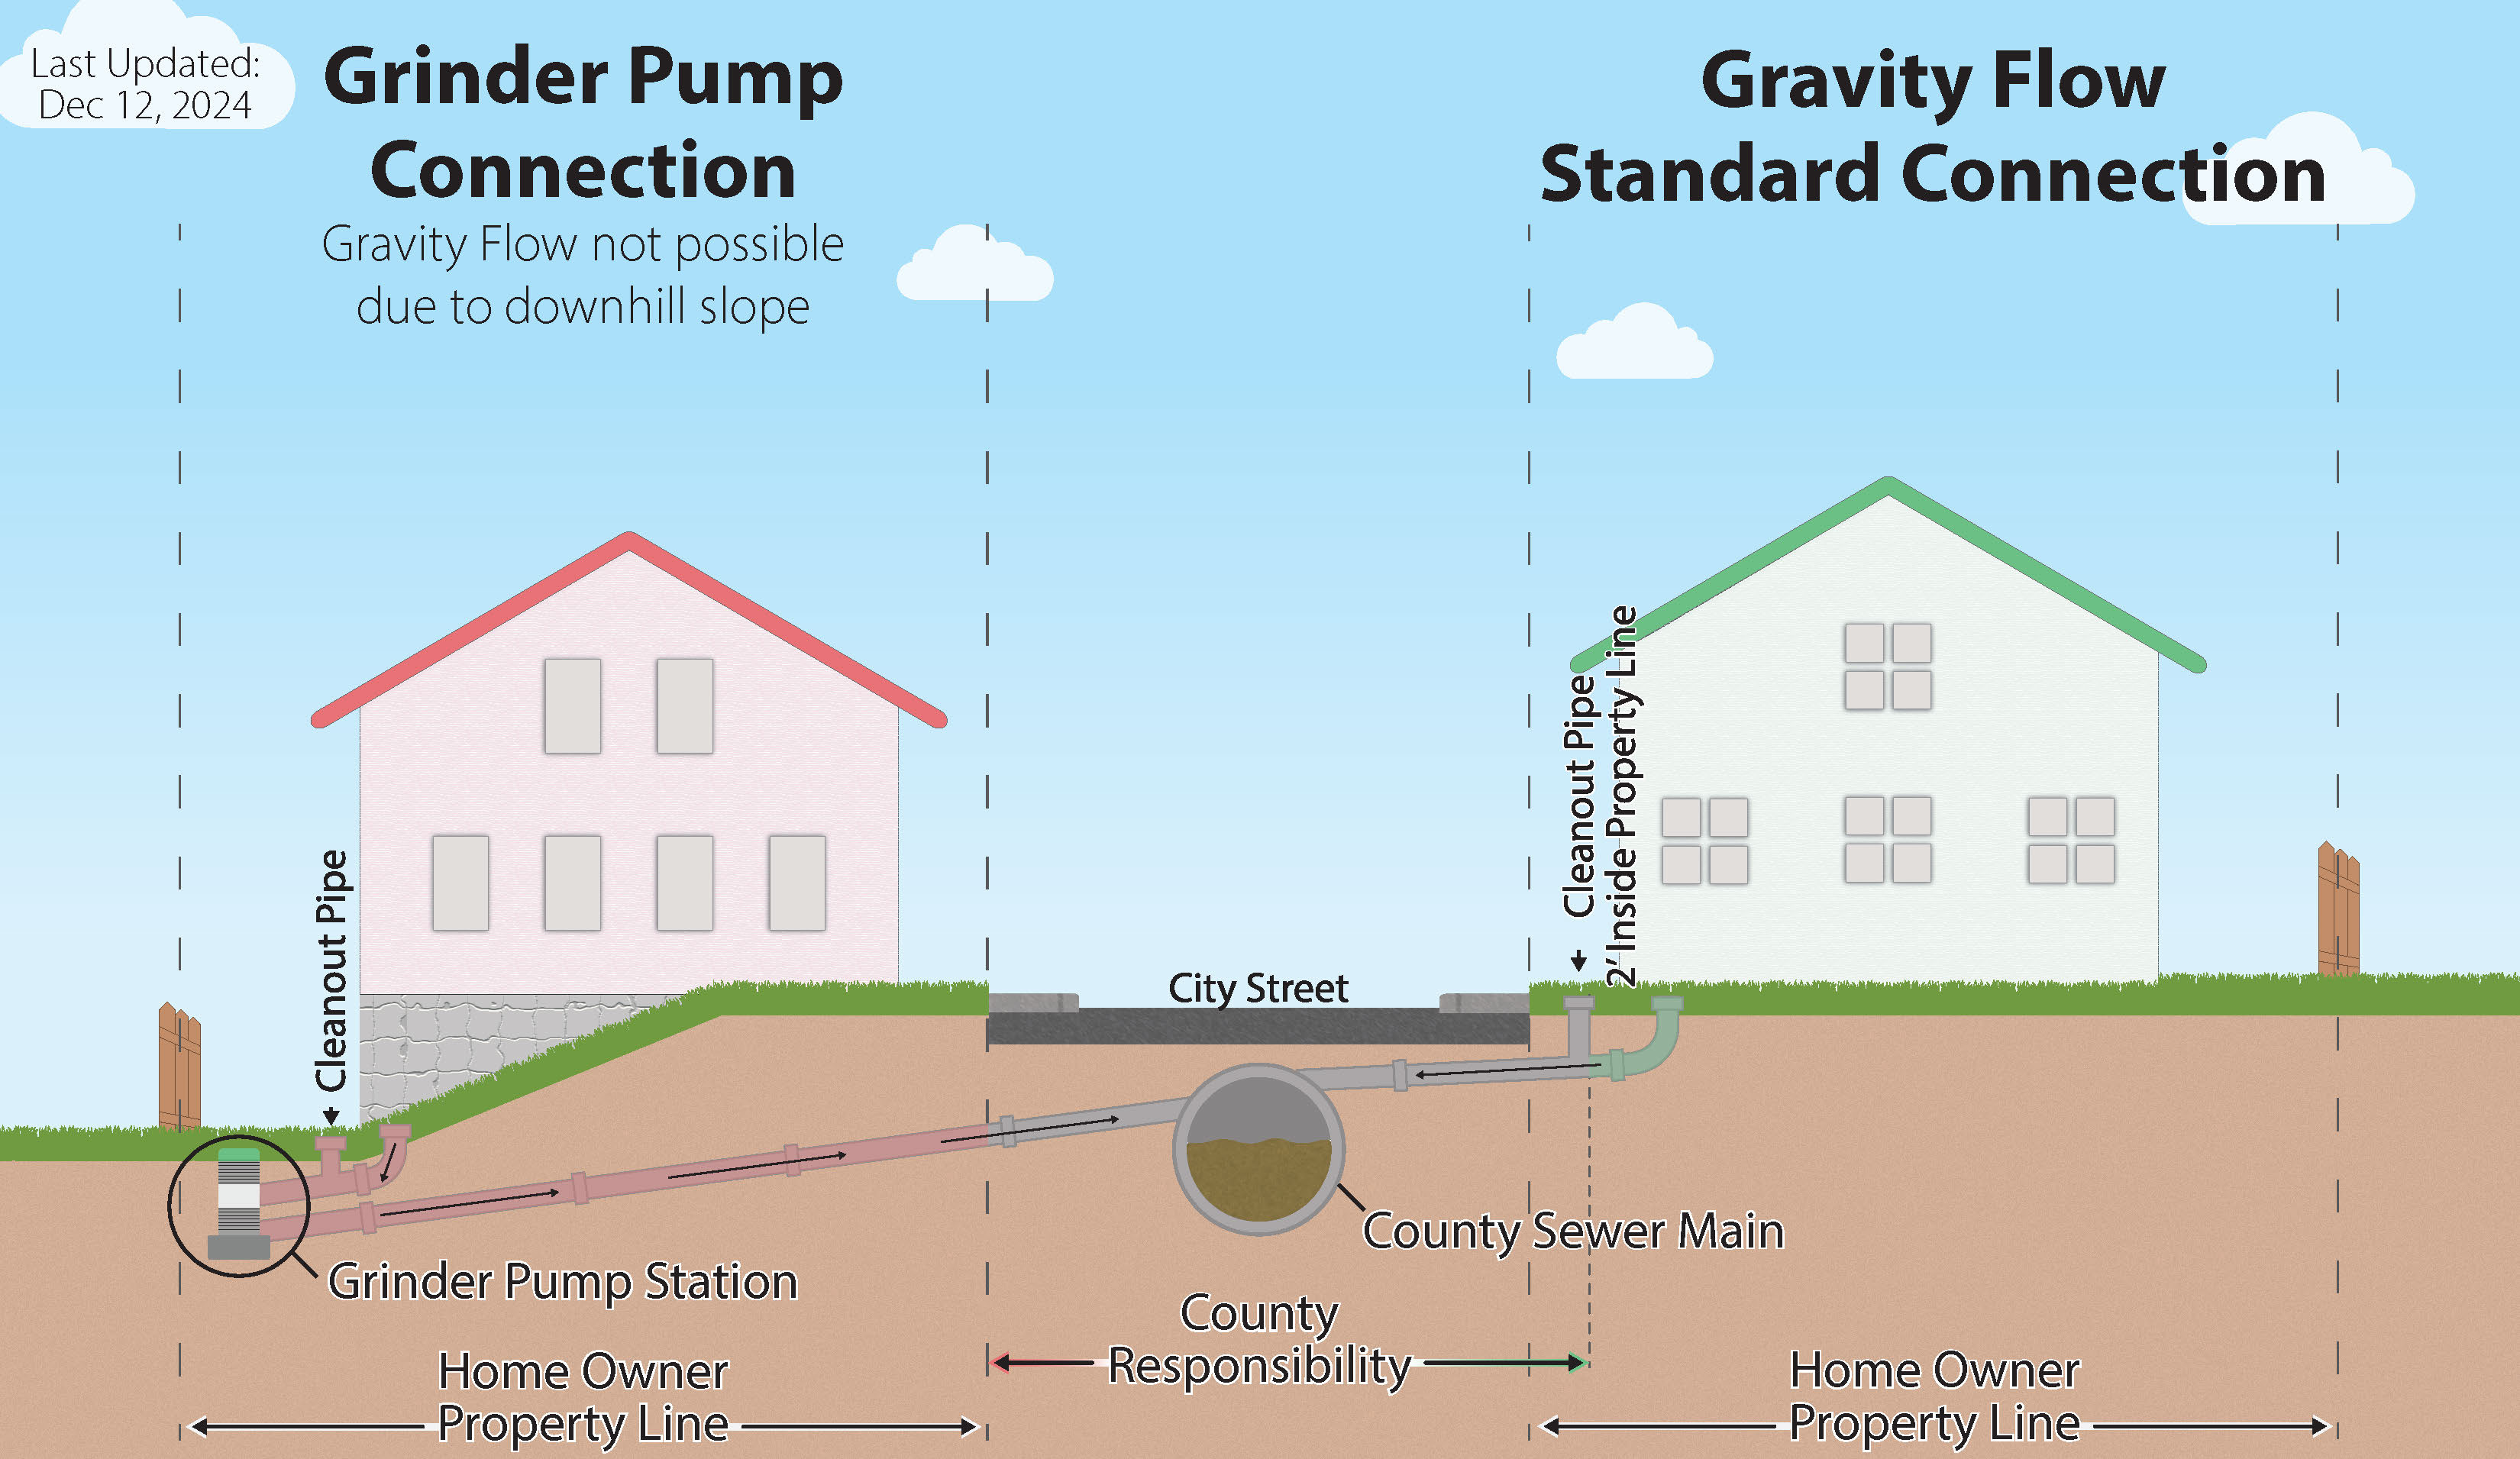
\includegraphics[width=0.9\textwidth]{alternative3a.jpg}
    \caption{Comparison of grinder-pump and gravity-flow connections showing how adequate elevation allows a standard gravity system while low terrain requires a pump installation~\cite{MauiRecovers_2024}.}
    \label{fig:alternative3a}
\end{figure}

\subsection{Typical Application in Practice}
Deep gravity systems are typically used when the ground elevation provides sufficient fall between the upstream service area and the outfall. These systems are ideal where excavation through stable soil layers is feasible and where long-term simplicity and low maintenance outweigh the higher initial construction cost.

\begin{figure}[H]
    \centering
    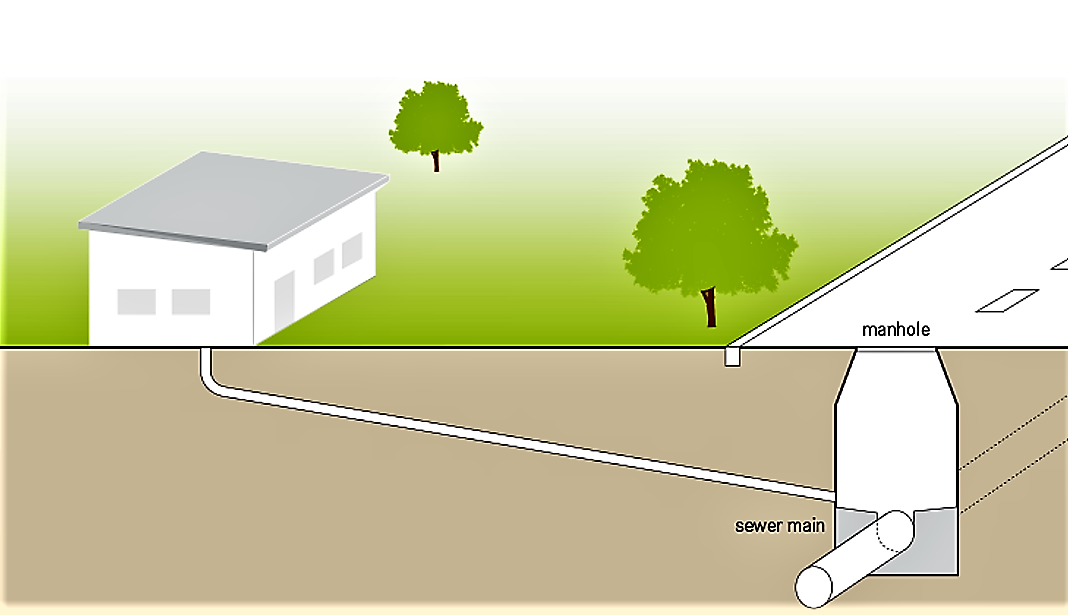
\includegraphics[width=0.85\textwidth]{alternative3b.png}
    \caption{Simplified cross-section of a deep gravity sewer showing pipe slope from a building connection to a manhole and main line under the roadway~\cite{Tilley_2014}.}
    \label{fig:alternative3b}
\end{figure}

\subsection{Advantages}
The primary advantage of the deep gravity sewer system lies in its simplicity and reliability. By relying entirely on gravitational flow, the system eliminates the need for pumps, electrical panels, or control mechanisms, significantly reducing operational complexity. Once constructed, the network operates passively and continuously, providing a dependable means of wastewater transport without requiring energy input. Because there are no moving parts, maintenance demands are limited to routine inspections and occasional cleaning of manholes, resulting in low life-cycle costs. The absence of mechanical equipment also ensures long-term reliability, as there are no mechanical failures that can disrupt service. Furthermore, the infrastructure remains fully underground, producing no visual or noise impact, which makes it highly acceptable to residential communities. From a sustainability perspective, this alternative promotes long-term energy conservation and minimizes the need for replacement parts or specialized operation.

\subsection{Disadvantages}
The main disadvantages of a deep gravity sewer system are associated with its high construction complexity and site limitations. Excavating to significant depths requires extensive labor, shoring, and dewatering, particularly in areas with weak or saturated soils where trench instability is a concern~\cite{Geotech_Colebrooke_2022}. These conditions not only increase construction time and cost but also introduce safety hazards that necessitate careful monitoring and support systems. Deep trenches may also conflict with existing or future utilities, such as water and gas lines, complicating coordination during both construction and maintenance. Repairs or new service connections at greater depths are considerably more difficult and expensive to perform, requiring specialized equipment and confined-space entry procedures. In some cases, topographic constraints may render this approach infeasible, particularly if the downstream sewer elevation is higher than the subdivision outlet~\cite{MDEQ_DesignGuidance_2025}. Overall, while deep gravity systems are operationally efficient once in place, their feasibility and cost-effectiveness are highly dependent on local soil conditions and elevation gradients.

\subsection{Technical, Economic, Environmental, and Social Considerations}
From a technical perspective, the deep gravity sewer offers a hydraulically simple and robust solution for wastewater conveyance. The flow relies solely on natural slope, making it inherently stable and resistant to operational interruptions. However, the design’s success depends heavily on precise surveying, soil strength, and groundwater conditions. Economically, deep gravity systems entail high initial capital investment due to excavation, shoring, and material costs, but their long-term operational and maintenance expenses are minimal compared to mechanical alternatives. Environmentally, the system operates without energy consumption and produces no emissions or noise once installed, posing minimal risk of spills or odors. The fully sealed pipeline and manhole network also reduce infiltration and exfiltration, preserving groundwater quality. From a social standpoint, this alternative is appealing because it eliminates above-ground equipment, visual clutter, and mechanical noise. Nonetheless, residents may experience temporary inconveniences during construction, such as road closures, vibrations, and hauling activities associated with deep trenching. In summary, while the deep gravity sewer represents the most sustainable and maintenance-free solution in the long term, it is only practical where favorable site topography and stable soil conditions exist.

\section{Final Selection}\label{sec:final_selection}

After a detailed evaluation of all three alternatives considering technical feasibility, constructability, cost, reliability, and long-term sustainability, the duplex submersible pump station with PVC force main was selected as the most appropriate option for the Colebrooke Subdivision wastewater conveyance system. This alternative best satisfies the design objectives established in the preliminary phase and meets both operational and regulatory requirements set forth by the Mississippi Department of Environmental Quality (MDEQ)~\cite{MDEQ_DesignGuidance_2025}.

The selected configuration demonstrates clear advantages in hydraulic performance and operational reliability. The existing topography of the subdivision does not provide sufficient elevation difference to sustain gravity flow throughout the service area, making a pumping solution essential. The duplex pump station ensures continuous operation by alternating between two pumps in a lead/lag cycle, maintaining stable discharge conditions and redundancy during maintenance or failure events. This arrangement aligns with common municipal practice for residential-scale lift stations and provides dependable performance under varying flow conditions~\cite{TenStates_RecommendedStandards_2014}.

From a constructability standpoint, the selected configuration allows installation at the natural low point of the subdivision with minimal excavation depth compared to deep gravity alternatives. The force main can be routed along the roadway corridor, allowing coordination with other infrastructure elements such as drainage and roadway construction. This integration simplifies construction sequencing and reduces overall site disturbance.

Maintenance and ownership considerations further support the selection of this centralized configuration. A single pump station allows for consolidated inspection, repair, and operational oversight by municipal staff. In contrast, a distributed grinder-pump network would require multiple individual service connections and private maintenance agreements, creating long-term management challenges. Centralized ownership under a municipal authority ensures consistent upkeep, protects public health, and maintains uniform service quality across all residences in the subdivision~\cite{EPA_LiftStation_DesignManual_2004}.

Economically, the centralized pump station provides a balanced solution over its service life. While the initial installation cost may be higher than some distributed alternatives, long-term operation and maintenance are simplified through centralized management and reduced system complexity. The use of standardized equipment and locally available components further supports cost-effective operation and maintenance~\cite{RSMeans_CostData_2025,ExcelFluidGroup_PumpComparison_2024}.

From an environmental and social perspective, the closed and pressurized nature of the force main minimizes the potential for infiltration, exfiltration, and odor generation. The below-grade installation reduces visual impacts and preserves the aesthetic character of the residential area. Collectively, these attributes contribute to sustainable infrastructure that supports public health, environmental protection, and community expectations for reliable wastewater management.

\section{Chapter Summary}\label{sec:chapter4_summary}

This chapter presented a comparative evaluation of three wastewater conveyance alternatives for the Colebrooke Subdivision: the duplex submersible pump station with PVC force main, the grinder pump and low-pressure sewer system, and the deep gravity sewer option. Each alternative was assessed in terms of hydraulic performance, constructability, cost, reliability, and environmental and social impacts. The analysis showed that the duplex submersible pump station provides the most balanced combination of technical feasibility, operational reliability, and economic efficiency. It satisfies the site’s hydraulic constraints, ensures centralized maintenance under municipal management, and offers long-term adaptability for future development. The findings of this analysis form the basis for the cost estimation and economic evaluation presented in the following chapter.

